\documentclass{article}


% if you need to pass options to natbib, use, e.g.:
%     \PassOptionsToPackage{numbers, compress}{natbib}
% before loading neurips_2023


% ready for submission
\usepackage{neurips_2023}


% to compile a preprint version, e.g., for submission to arXiv, add add the
% [preprint] option:
%     \usepackage[preprint]{neurips_2023}


% to compile a camera-ready version, add the [final] option, e.g.:
%     \usepackage[final]{neurips_2023}


% to avoid loading the natbib package, add option nonatbib:
%    \usepackage[nonatbib]{neurips_2023}


\usepackage[utf8]{inputenc} % allow utf-8 input
\usepackage[T1]{fontenc}    % use 8-bit T1 fonts
\usepackage{hyperref}       % hyperlinks
\usepackage{url}            % simple URL typesetting
\usepackage{booktabs}       % professional-quality tables
\usepackage{amsfonts}       % blackboard math symbols
\usepackage{nicefrac}       % compact symbols for 1/2, etc.
\usepackage{microtype}      % microtypography
\usepackage{xcolor}         % colors
\usepackage[noend]{algpseudocode}
\usepackage{algorithm}
\usepackage{amsmath,amsfonts,amssymb}
\usepackage{graphicx} % Include this line in the preamble


\title{Adaptive Group Normalization: Harnessing Dynamic Channel Statistics for Enhanced Deep Learning Performance}


% The \author macro works with any number of authors. There are two commands
% used to separate the names and addresses of multiple authors: \And and \AND.
%
% Using \And between authors leaves it to LaTeX to determine where to break the
% lines. Using \AND forces a line break at that point. So, if LaTeX puts 3 of 4
% authors' names on the first line, and the last on the second line, try using
% \AND instead of \And before the third author name.


\author{
  Yair Smadar\thanks{Use footnote for providing further information
    about the author (webpage, alternative address)---\emph{not} for acknowledging
    funding agencies.} \\
  School of Computer Science\\
  Ariel University\\
  \texttt{yair.smadar1@gmail.com} \\
  % examples of more authors
  \And
  Assaf Hoogi \\
  School of Computer Science\\
  Ariel University\\
  \texttt{assafh@ariel.ac.il} \\
  % \texttt{email} \\
  % \AND
  % Coauthor \\
  % Affiliation \\
  % Address \\
  % \texttt{email} \\
  % \And
  % Coauthor \\
  % Affiliation \\
  % Address \\
  % \texttt{email} \\
  % \And
  % Coauthor \\
  % Affiliation \\
  % Address \\
  % \texttt{email} \\
}


\begin{document}


\maketitle


\begin{abstract}
Adaptive Group Normalization (AGN) introduces a dynamic approach to neural network normalization, clustering channels based on statistical properties through an adapted clustering algorithm. This method surpasses Group Normalization (GN) by enabling variable group sizes and aligning channels with similar statistics for more effective normalization. AGN enhances model adaptability and accuracy by providing flexible normalization that can be tailored to specific characteristics of the data, leading to improved learning dynamics. Furthermore, AGN's ability to dynamically adjust to the changing distribution of features within a network promotes more stable and faster convergence, offering significant advancements in deep learning and computer vision. This adaptability is particularly advantageous in scenarios where GN's fixed group sizes limit performance, making AGN a promising alternative for a wide range of applications. Our experiments on classification, object detection, and segmentation tasks across benchmark datasets and architectures underscore AGN's superiority over GN.
\end{abstract}


\section{Introduction}
In the realm of deep learning, stabilizing and accelerating model training are critical goals, achieved notably through various normalization techniques. Batch Normalization (BN) is favored for its efficiency in large-batch scenarios, Layer Normalization (LN) excels in recurrent neural networks and is also the current preferred normalization in various Transformers architectures. Instance Normalization (IN) is preferred in style transfer applications, and Group Normalization (GN) is advantageous for tasks with smaller batch sizes or where BN's dependence on batch size is limiting. Each technique offers unique benefits tailored to specific settings, yet the quest for more adaptable and efficient normalization methods continues.

Adaptive Group Normalization (AGN) emerges as a pioneering approach, refining the concept of GN (See figure \ref{fig:norm_methods}). AGN dynamically clusters channels based on their statistical properties, allowing for variable group sizes and a more tailored normalization process. Unlike traditional methods, AGN's groups are determined not by arbitrary divisions but by the inherent statistics of the channels, ensuring a more natural and effective normalization. This novel mechanism enables AGN to adaptively optimize group configurations for enhanced model convergence, filling a gap left by existing normalization techniques.

The primary objective of AGN is to markedly improve model convergence. By leveraging channel statistics for group formation, AGN introduces a level of adaptability previously unseen in normalization practices. This approach ensures that normalization is closely aligned with the data's statistical characteristics, optimizing the training process.

AGN's methodology involves performing clustering on the first minibatch of each normalization layer every \(x\) epochs. This clustering utilizes a 2D representation of each channel's mean and variance, grouping channels based on these statistical metrics. The resulting groups, which may vary in size, are then normalized individually. Among various clustering techniques evaluated, K-means coupled with an Isolation Forest algorithm for outlier removal has proven most effective in our experiments.

The contributions of this paper are multifaceted. Firstly, AGN introduces a flexible, data-driven approach to normalization, enhancing model performance and convergence. Secondly, by adapting group sizes according to data statistics, AGN provides a novel solution to the limitations of fixed group sizes in GN. Lastly, our comprehensive experiments across several deep learning tasks demonstrate AGN's superior performance over traditional normalization methods, showcasing its potential to significantly advance the field of neural network training.

\begin{figure}
  \centering
  {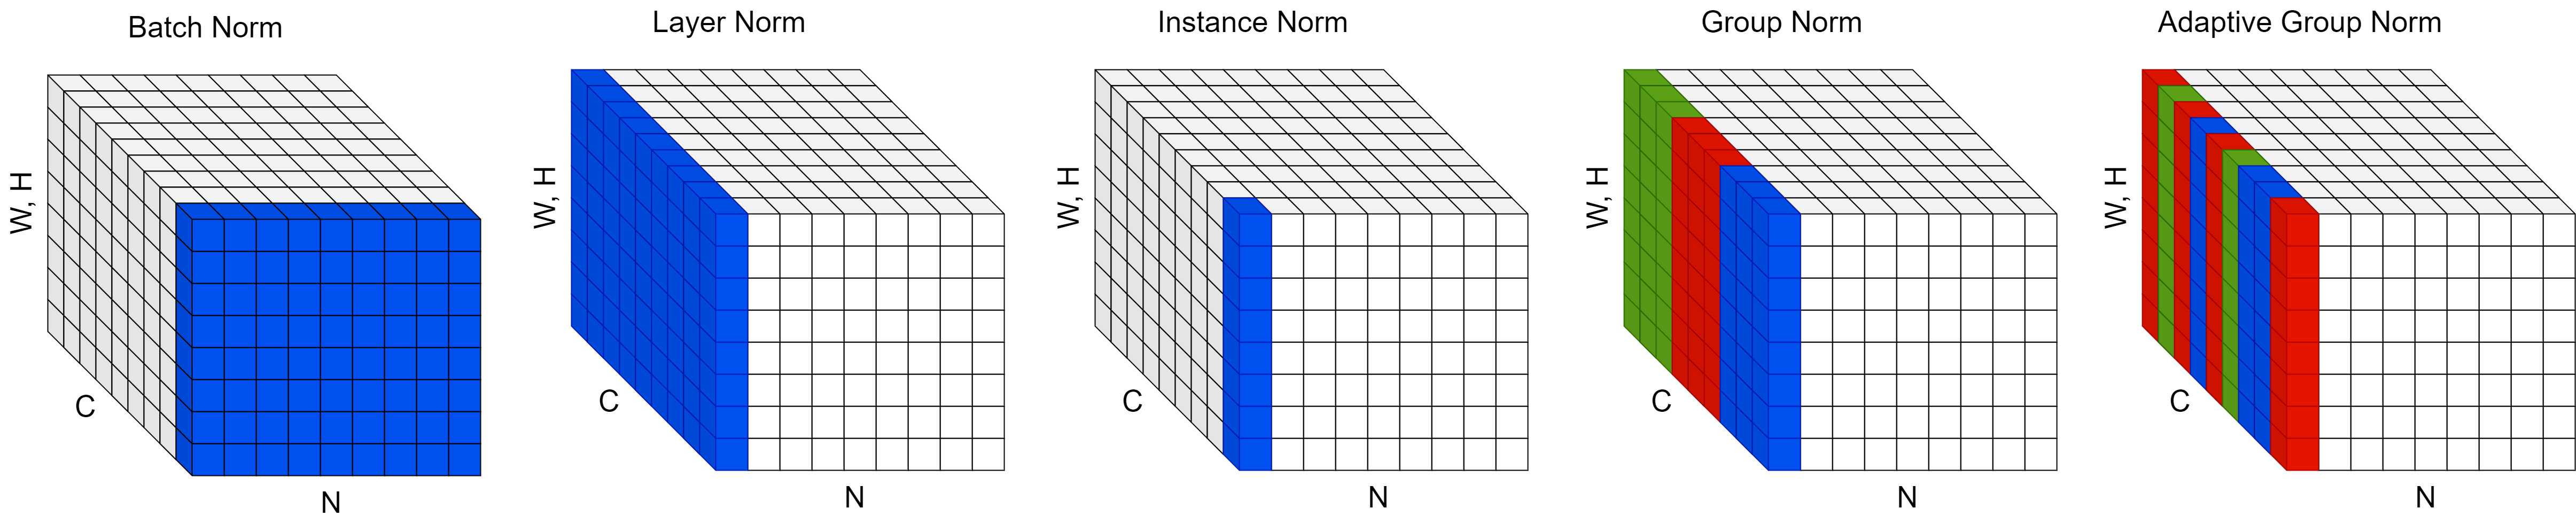
\includegraphics[width=13cm]{images/Normaliozations blocks.drawio.png}} 
  \caption{\textbf{Normalization methods.} Each subplot represents a feature map tensor, where \( N \) denotes the batch axis, \( C \) the channel axis, and \( (H, W) \) the spatial axes. The pixels highlighted in colors are standardized by a shared mean and variance, calculated by pooling their values.}
    \label{fig:norm_methods}
\end{figure}

\section{Related work}
The advent of normalization techniques has significantly influenced the field of deep learning, enhancing model training efficiency and stability. This section delves into the principal normalization methods, underscoring their unique contributions and limitations, thereby setting the stage for the introduction of Adaptive Group Normalization (AGN).

\paragraph{Batch Normalization (BN)}
Introduced by Ioffe and Szegedy (2015), Batch Normalization has become a cornerstone in neural network training, aimed at addressing internal covariate shift. By normalizing the inputs of each layer across the batch dimension, BN accelerates training and enables the use of higher learning rates. Despite its widespread adoption, BN's dependence on batch size poses limitations in scenarios where small batches are preferable or necessary, such as limited memory resources or sequence-based tasks.
\paragraph{Layer Normalization (LN)}
Ba et al. (2016) proposed Layer Normalization as an alternative to BN, normalizing across the features of a single layer. LN's independence from batch size makes it particularly suited for recurrent neural networks and tasks with dynamic batch sizes. However, LN does not account for batch-wise statistics, which can be beneficial in tasks with stable data distributions across batches.
\paragraph{Instance Normalization (IN)}
Instance Normalization, introduced by Ulyanov et al. (2016), targets style transfer applications. By normalizing each channel in each data instance, IN allows models to focus on style features, improving the quality of generated images. Though effective in specific contexts, IN's application is limited outside tasks where instance-level normalization is beneficial.
\paragraph{Group Normalization (GN)}
Wu and He (2018) presented Group Normalization as a versatile normalization technique that divides channels into groups and normalizes these groups independently. GN's effectiveness is not contingent on batch size, making it valuable in a wide array of tasks, especially those involving small batches or highly variable data. However, GN's static grouping mechanism does not account for the dynamic nature of data statistics, which can lead to suboptimal normalization in complex models.

\paragraph{Power Normalization (PowerNorm)}
Power Normalization (PowerNorm) proposes an approach aimed at enhancing the training stability and performance of deep neural networks for NLP tasks. While specific details of PowerNorm's methodology may vary, its core principle involves adjusting the normalization process to be more adaptive to the power distribution of the activations within a network. This adaptability ensures that the normalization effect is consistently beneficial across different layers and architectures, potentially addressing the challenges of internal co-variate shift and training efficiency more effectively than its predecessors.
PowerNorm is designed to complement the strengths and mitigate the weaknesses of BN by offering a more dynamic normalization strategy.

\paragraph{Switchable Normalization (SwitchNorm)}
Switchable Normalization (SwitchNorm) offers a flexible approach to normalization by dynamically selecting between Batch Normalization, Instance Normalization, and Layer Normalization within a single framework. This method, introduced by Luo et al., is designed to leverage the strengths of each normalization technique, adapting to various data distributions and training conditions. SwitchNorm adjusts its normalization strategy based on the specific requirements of the task and the dataset, potentially offering superior generalization across different neural network architectures and applications.


% \paragraph{Spectral Normalization}
% Spectral Normalization, proposed by Miyato et al., specifically targets the stabilization of training in Generative Adversarial Networks (GANs) by normalizing the spectral norm of the weight matrices in the network. This technique ensures the Lipschitz continuity of the network functions, leading to more stable training dynamics and improved generation quality. Spectral Normalization has since been applied beyond GANs, proving to be an effective regularization method for various deep learning models to promote smoother optimization landscapes.
% \paragraph{Cosine Normalization}
% Cosine Normalization introduces a novel perspective on normalization by scaling the weights and inputs of a network based on the cosine similarity between them. This approach, focusing on the angle between the weight vector and the input vector, aims to enhance the learning process by ensuring that the scale of the weights does not dominate the training dynamics. Cosine Normalization has shown promise in reducing the sensitivity of the network to the scale of weights and inputs, potentially improving robustness and generalization.
% \paragraph{Weight Normalization}
% Weight Normalization, developed by Salimans and Kingma, is a technique that decouples the magnitude of the weights from their direction, by normalizing the weight vectors. This simplifies the optimization landscape, leading to faster convergence and potentially improving training performance. Weight Normalization is particularly beneficial in the context of recurrent neural networks and variational inference, where it can significantly enhance training efficiency and stability.


In summary, while existing normalization techniques have individually advanced the field of neural network training, they also present specific limitations that AGN seeks to address. Through its innovative approach to dynamic channel grouping, AGN represents a significant step forward, potentially redefining normalization practices in deep learning.

\section{Adaptive group normalization}
Adaptive Group Normalization (AGN) proposes a novel dynamic approach to enhance the efficacy of deep learning models through the strategic exploitation of the statistical characteristics inherent in network channels. This methodology is underpinned by two principal components: the AGN scheduler and the channel re-clustering mechanism.

\subsection{AGN Scheduler}
The AGN scheduler serves as an autonomous system engineered to ascertain the optimal junctures for channel re-clustering, predicated on their statistical attributes. The scheduler's decision-making paradigm is governed by multiple parameters:

\begin{enumerate}
    \item The designated epoch for initiating the first clustering (\(E_{init}\)).
    \item The epoch intervals designated for subsequent re-clustering events (\(E_{interval}\)). This regimen is meticulously applied to each AGN layer within the initial mini-batch of the corresponding epoch. The rationale behind this strategy is predicated on the hypothesis that each filter, by engendering a new channel, aligns the output within a uniform statistical framework.
    \item Maximum re-clustering epoch, Marks in which epoch to stop performing channel re-clustering, and stay with the last established channel clusters (\(E_{max}\)).
\end{enumerate}

Empirical analyses advocate that an interval setting of \(E_{init} = 0\), \(E_{interval} = 20\) and \(E_{max} = 50\) is conducive to achieving optimal outcomes.

\subsection{Reclustering Channels}
The re-clustering mechanism is articulated as follows:

\begin{enumerate}
    \item For every channel within the mini-batch, the statistical attributes are computed as \[(statics_i = (\mu_{channel_i}, \sigma^2_{channel_i}))\], wherein \(\mu_{channel_i}\) and \(\sigma^2_{channel_i}\) represent the mean and variance of the \(i\)-th channel, respectively.
    
    \item An outlier detection algorithm, exemplified by IsolationForest, is employed to excise outliers from the set \[Statics = \{ statics_0, statics_1, \ldots, statics_n \}\].

    
    \item Subsequent to outlier removal, the mean (\(\mu_{C_i}\)) and variance (\(\sigma^2_{C_i}\)) for the residual channels are recalculated, with \(C_i\) denoting the \(i\)-th channel in each image of the mini-batch.
    
    \item Given a batch size denoted as \((N, C, H, W)\), this procedure culminates in \(C\) points of \((\mu_{C_i}, \sigma^2_{C_i})\).
    
    \item The KMeans algorithm is subsequently utilized to cluster the \(C\) points into \(G\) unique groups, where \(G\) is a predetermined parameter specifying the number of groups and aligns with the GN parameter. This process results in the creation of channel clusters, denoted as \(K\).
\end{enumerate}

\subsection{Normalization According to the clustering results}
In the course of training, as data traverses through the normalization layer, channels are apportioned into groups in alignment with \(K\), with each group undergoing normalization in conformity with established norms. Analogous to Group Normalization (GN), AGN incorporates learnable parameters \(\alpha\) and \(\beta\) for each channel, which are iteratively updated in a process akin to that of GN.

This meticulously structured paradigm of dynamic channel normalization, encapsulated by AGN, significantly refines the training process. It achieves this by judiciously adjusting the normalization groups in response to the evolving statistical dynamics of the data, thereby substantially enhancing model convergence and performance.


\begin{algorithm}
\caption{Adaptive Group Normalization Procedure}
\begin{algorithmic}[1]
\State \textbf{Input:} Input mini-batch $X \in \mathbb{R}^{N \times C \times H \times W}$, epoch count $E$, initial clustering epoch $E_{init}$, clustering interval $E_{interval}$, maximum re-clustering $E_{max}$, number of target groups $G$.
\State \textbf{Output:} Normalized output tensor $Y$.

\Procedure{ScheduleClustering}{$E, E_{init}, E_{interval}, E_{max}$}
    \If{($E_{init} <= E <= E_{max}$  \textbf{and} $(E - E_{init}) \mod E_{interval} = 0$)}
        \State Invoke \Call{ReclusterChannels}{}
    \Else
        \State Invoke \Call{NormalizeChannels}{}
    \EndIf
\EndProcedure

\Procedure{ReclusterChannels}{$X, G$}
    \For{each channel $i \in \{1, \ldots, C*N\}$} \Comment{$N=Batch size, C=\#channels$}
        \State Compute $statics_i = \left(\mu_{channel_i}, \sigma^2_{channel_i}\right)$. 
    \EndFor
    \State Apply IsolationForest on $\{ statics_0, statics_1, \ldots, statics_{N*C} \}$ for outlier removal.
    \State For non-outlier channels, recalculate $\mu_{C_i}$ and $\sigma^2_{C_i}$ for each $i \in C$.
    \State Employ KMeans to partition $C$ points into $G$ clusters, yielding grouping $K$.
    \State Invoke \Call{NormalizeChannels}{}
\EndProcedure

\Procedure{NormalizeChannels} {$X, K$}
    \For{each cluster $k \in K$}
        \State Partition $X$ according to cluster assignments in $k$.
        \State Normalize each partitioned group following GN principles.
    \EndFor
    \State \textbf{return} Normalized output $Y$.
\EndProcedure

\end{algorithmic}
\end{algorithm}

\section{Theoretical Background}
In deep learning, normalization techniques play a crucial role in stabilizing the training process, enhancing convergence, and improving model performance. The strategy of normalizing channels based on closely aligned statistical properties—specifically, mean and variance—derives from mathematical and empirical insights that underscore its benefits for deep learning architectures. Here, we provide the theory for the effectiveness of this approach.

\subsection{Reduction of Internal Covariate Shift}
Internal Covariate Shift refers to the phenomenon where the distribution of network layer inputs changes during training, complicating the learning process. By normalizing channels with similar statistical properties, the consistency in the distribution of inputs across layers is maintained. Mathematically, if the inputs to a layer are normalized to have consistent mean \(\mu\) and variance \(\sigma^2\), the layer's weights can be updated more effectively, reducing internal covariate shift and facilitating faster convergence.

\subsubsection{Mathematical Basis for Effective Weight Updates}

Given a normalized input \(\hat{x}_i\) for each input \(x_i\), normalization transforms \(x_i\) as follows:

\[
\hat{x}_i = \frac{x_i - \mu}{\sqrt{\sigma^2 + \epsilon}}
\]

where \(\epsilon\) is a small constant for numerical stability. This transformation standardizes the inputs, leading to a more stable distribution across layers.

The gradient of the loss function \(L\) with respect to the weights \(W\), denoted by \(\frac{\partial L}{\partial W}\), plays a crucial role in the backpropagation algorithm. For a layer receiving normalized inputs, the gradient with respect to a weight \(w_{ij}\) can be expressed using the chain rule as:

\[
\frac{\partial L}{\partial w_{ij}} = \sum_k \left( \frac{\partial L}{\partial \hat{x}_k} \frac{\partial \hat{x}_k}{\partial w_{ij}} \right)
\]

Normalization ensures the gradient \(\frac{\partial L}{\partial w_{ij}}\) remains stable, facilitating smoother optimization landscapes and more consistent weight updates.

\subsubsection{Advantages of Variable Group Normalization Over Group Normalization}

While GN divides channels into fixed groups for normalization, VGN adapts the group sizes based on the data's statistical properties. This adaptability offers several benefits:

\begin{itemize}
    \item \textbf{Adaptability to Data Distribution:}
    VGN dynamically adjusts groups to align with the statistical properties of the inputs, optimizing the normalization process. The optimal number of groups \(G^*\) can be determined by minimizing the within-group variance:
    \[
    G^* = \arg\min_G \sum_{g=1}^G \text{Var}(\text{Group}_g)
    \]

    \item \textbf{Improved Optimization Landscape:}
    By fine-tuning the normalization to the current state of the network, VGN reduces internal covariate shift more effectively than GN, promoting faster convergence:
    \[
    \Delta w_{ij} \propto -\eta \frac{\partial L}{\partial w_{ij}} = -\eta \sum_k \left( \frac{\partial L}{\partial \hat{x}_k} \frac{\partial \hat{x}_k}{\partial w_{ij}} \right)
    \]

    \item \textbf{Flexibility Across Architectures and Tasks:}
    VGN's mathematical flexibility allows it to be applied more universally without the need for manual tuning of group sizes, unlike GN.
\end{itemize}


\subsection{Enhanced Learning Dynamics}
Normalizing channels with close statistics ensures that the scale of inputs to activation functions remains relatively consistent. This is particularly important for nonlinear activation functions like ReLU, which can suffer from saturation or the "dead neuron" problem with highly variable input scales. For an activation function \(f(x)\) and an input \(x\) normalized as \(x' = \frac{x - \mu}{\sqrt{\sigma^2 + \epsilon}}\), where \(\epsilon\) is a small constant for numerical stability, such normalization helps maintain efficient gradient-based learning by preventing extreme input values.

\subsection{Improved Generalization}
Channels with similar statistical properties are likely detecting similar features in the input data. Grouping and normalizing these channels together can sharpen the model's feature detection capabilities, as normalization minimizes noise and variance. Mathematically, this approach simplifies the hypothesis space explored during training, aiding the model in generalizing well to unseen data by reducing the complexity of the space.

\subsection{Stability in Gradient Propagation}
Stable gradient propagation is essential, especially in deep networks where vanishing or exploding gradients can impede learning. Normalizing channels by their statistics contributes to this stability. Let \(\frac{\partial L}{\partial x}\) represent the gradient of the loss function with respect to a layer's inputs. Normalization ensures that these inputs, \(x\), exhibit reduced variance, thereby preventing extreme gradient values and promoting stable updates across the network's layers.

In summary, normalizing channels based on their statistical properties addresses key challenges in deep learning through mathematical principles, leading to more efficient, stable, and effective training processes. This strategy not only aids in achieving faster convergence but also improves the model's ability to learn and generalize, highlighting the significance of such normalization techniques in deep learning models.


\section{Experiments}
\begin{table}
  \caption{This table showcases classification accuracy for VGN, SGN, and GN across architectures, with top results in \textbf{bold}. GN performances align with the literature for models trained anew.}
  \label{classification results - Init weight 0}
  \centering
  \begin{tabular}{lllll}
    \toprule
    \multicolumn{4}{r}{Test accuracy - Init weight 0}                   \\
    \cmidrule(r){3-5}
    Dataset     & Architecture     & VGN & SGN & GN \\
    \midrule
    CIFAR100 & ResNet50  & 65.85 & \textbf{68.02} & 66.73    \\
    CIFAR100 & MobileNetV2  & \textbf{69.97} & 69.86 & 69.02 \\
    CIFAR100 & EfficientNet-b0  & 72.94 & \textbf{73.09} & 72.4    \\
    CIFAR100 & DenseNet-121  & \textbf{69.26} & 69.38 & 68.44    \\
    CIFAR100 & RevVit Transformer  & 52.11 & 52.07 & \textbf{52.8}    \\
    \bottomrule
  \end{tabular}
\end{table}

\begin{table}
  \caption{This table showcases classification accuracy for VGN, SGN, and GN across architectures, with top results in \textbf{bold}. GN performances align with the literature for models trained anew.}
  \label{classification results - Init weight 1}
  \centering
  \begin{tabular}{lllll}
    \toprule
    \multicolumn{4}{r}{Test accuracy - Init weight 1}                   \\
    \cmidrule(r){3-5}
    Dataset     & Architecture     & VGN & SGN & GN \\
    \midrule
    CIFAR100 & ResNet50  & 64.56 & \textbf{67.14} & 65.89    \\
    CIFAR100 & MobileNetV2  & \textbf{69.86} & 69.64 & 67.57 \\
    CIFAR100 & EfficientNet-b0  & \textbf{72.62} & 72.54 & 71.85    \\
    CIFAR100 & DenseNet-121  & \textbf{69.73} & 69.55 & 68.84    \\
    CIFAR100 & RevVit Transformer  & 52.65 & 52.65 & \textbf{54.61}    \\
    \bottomrule
  \end{tabular}
\end{table}

\begin{table}
  \caption{This table showcases classification accuracy for VGN, SGN, and GN across architectures, with top results in \textbf{bold}. GN performances align with the literature for models trained anew.}
  \label{classification results - Init weight 2}
  \centering
  \begin{tabular}{lllll}
    \toprule
    \multicolumn{4}{r}{Test accuracy - Init weight 2}                   \\
    \cmidrule(r){3-5}
    Dataset     & Architecture     & VGN & SGN & GN \\
    \midrule
    CIFAR100 & ResNet50  & - & - & -    \\
    CIFAR100 & MobileNetV2  & \textbf{70.04} & 68.53 & 68.46 \\
    CIFAR100 & EfficientNet-b0  & \textbf{72.78} & 72.45 & 72.12    \\
    CIFAR100 & DenseNet-121  & - & 68.84 & 68.68    \\
    CIFAR100 & RevVit Transformer  & - & - & -    \\
    \bottomrule
  \end{tabular}
\end{table}


\begin{figure}
  \centering
  \fbox{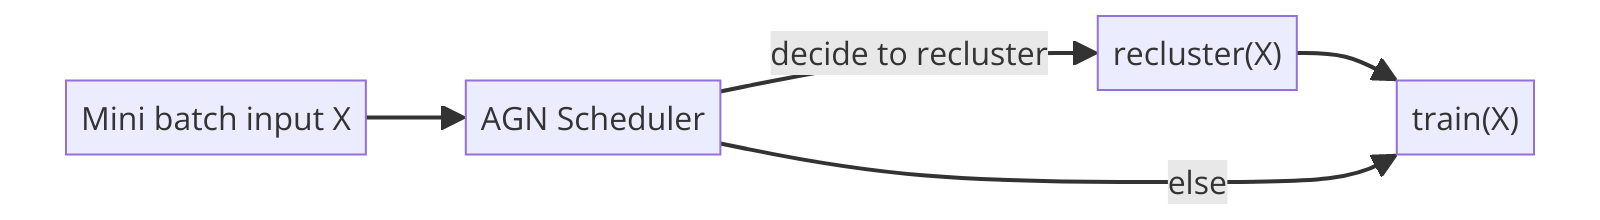
\includegraphics[width=13cm]{images/diagram.png}} 
  \caption{\textbf{AGN Scheduler}}
  \label{fig:agn_scheduler}
\end{figure}


\subsection{Tables}

All tables must be centered, neat, clean, and legible.  The table number and
title always appear before the table.  See Table~\ref{sample-table}.


Note that publication-quality tables \emph{do not contain vertical rules.} We
strongly suggest the use of the \verb+booktabs+ package, which allows for
typesetting high-quality, professional tables:
\begin{center}
  \url{https://www.ctan.org/pkg/booktabs}
\end{center}
This package was used to typeset Table~\ref{sample-table}.


\subsection{Math}
Note that displaying math in bare TeX commands will not create correct line numbers for submission. Please use LaTeX (or AMSTeX) commands for unnumbered display math. (You really shouldn't be using \$\$ anyway; see \url{https://tex.stackexchange.com/questions/503/why-is-preferable-to} and \url{https://tex.stackexchange.com/questions/40492/what-are-the-differences-between-align-equation-and-displaymath} for more information.)

\subsection{Final instructions}

Do not change any aspects of the formatting parameters in the style files.  In
particular, do not modify the width or length of the rectangle the text should
fit into, and do not change font sizes (except perhaps in the
\textbf{References} section; see below). Please note that pages should be
numbered.


\section{Preparing PDF files}


Please prepare submission files with paper size ``US Letter,'' and not, for
example, ``A4.''


Fonts were the main cause of problems in the past years. Your PDF file must only
contain Type 1 or Embedded TrueType fonts. Here are a few instructions to
achieve this.


\begin{itemize}


\item You should directly generate PDF files using \verb+pdflatex+.


\item You can check which fonts a PDF files uses.  In Acrobat Reader, select the
  menu Files$>$Document Properties$>$Fonts and select Show All Fonts. You can
  also use the program \verb+pdffonts+ which comes with \verb+xpdf+ and is
  available out-of-the-box on most Linux machines.


\item \verb+xfig+ "patterned" shapes are implemented with bitmap fonts.  Use
  "solid" shapes instead.


\item The \verb+\bbold+ package almost always uses bitmap fonts.  You should use
  the equivalent AMS Fonts:
\begin{verbatim}
   \usepackage{amsfonts}
\end{verbatim}
followed by, e.g., \verb+\mathbb{R}+, \verb+\mathbb{N}+, or \verb+\mathbb{C}+
for $\mathbb{R}$, $\mathbb{N}$ or $\mathbb{C}$.  You can also use the following
workaround for reals, natural and complex:
\begin{verbatim}
   \newcommand{\RR}{I\!\!R} %real numbers
   \newcommand{\Nat}{I\!\!N} %natural numbers
   \newcommand{\CC}{I\!\!\!\!C} %complex numbers
\end{verbatim}
Note that \verb+amsfonts+ is automatically loaded by the \verb+amssymb+ package.


\end{itemize}


If your file contains type 3 fonts or non embedded TrueType fonts, we will ask
you to fix it.


\subsection{Margins in \LaTeX{}}


Most of the margin problems come from figures positioned by hand using
\verb+\special+ or other commands. We suggest using the command
\verb+\includegraphics+ from the \verb+graphicx+ package. Always specify the
figure width as a multiple of the line width as in the example below:
\begin{verbatim}
   \usepackage[pdftex]{graphicx} ...
   \includegraphics[width=0.8\linewidth]{myfile.pdf}
\end{verbatim}
See Section 4.4 in the graphics bundle documentation
(\url{http://mirrors.ctan.org/macros/latex/required/graphics/grfguide.pdf})


A number of width problems arise when \LaTeX{} cannot properly hyphenate a
line. Please give LaTeX hyphenation hints using the \verb+\-+ command when
necessary.


\begin{ack}
Use unnumbered first level headings for the acknowledgments. All acknowledgments
go at the end of the paper before the list of references. Moreover, you are required to declare
funding (financial activities supporting the submitted work) and competing interests (related financial activities outside the submitted work).
More information about this disclosure can be found at: \url{https://neurips.cc/Conferences/2023/PaperInformation/FundingDisclosure}.


Do {\bf not} include this section in the anonymized submission, only in the final paper. You can use the \texttt{ack} environment provided in the style file to autmoatically hide this section in the anonymized submission.
\end{ack}



\section{Supplementary Material}

Authors may wish to optionally include extra information (complete proofs, additional experiments and plots) in the appendix. All such materials should be part of the supplemental material (submitted separately) and should NOT be included in the main submission.


\section*{References}


References follow the acknowledgments in the camera-ready paper. Use unnumbered first-level heading for
the references. Any choice of citation style is acceptable as long as you are
consistent. It is permissible to reduce the font size to \verb+small+ (9 point)
when listing the references.
Note that the Reference section does not count towards the page limit.
\medskip


{
\small


[1] Alexander, J.A.\ \& Mozer, M.C.\ (1995) Template-based algorithms for
connectionist rule extraction. In G.\ Tesauro, D.S.\ Touretzky and T.K.\ Leen
(eds.), {\it Advances in Neural Information Processing Systems 7},
pp.\ 609--616. Cambridge, MA: MIT Press.


[2] Bower, J.M.\ \& Beeman, D.\ (1995) {\it The Book of GENESIS: Exploring
  Realistic Neural Models with the GEneral NEural SImulation System.}  New York:
TELOS/Springer--Verlag.


[3] Hasselmo, M.E., Schnell, E.\ \& Barkai, E.\ (1995) Dynamics of learning and
recall at excitatory recurrent synapses and cholinergic modulation in rat
hippocampal region CA3. {\it Journal of Neuroscience} {\bf 15}(7):5249-5262.
}

%%%%%%%%%%%%%%%%%%%%%%%%%%%%%%%%%%%%%%%%%%%%%%%%%%%%%%%%%%%%


\end{document}